\chapter{Proposta}


A adoção de padrões é uma premissa básica para o desenvolvimento de software, pois ao trabalhar com variações dentro de uma organização, a tendência é gerar confusão. Assim, o objetivo do ModMan é projetar e implementar um módulo padrão de permissões de acesso, de modo que o mesmo possa ser utilizado por diferentes plataformas, como desktop, Web e mobile, eliminando assim este módulo do desenvolvimento de um software e utilizando o trabalho proposto como um SaaS provedor das permissões do software cliente a ser desenvolvido.


É comum encontrar frameworks de desenvolvimento de software que automatizam a geração de esquemas de configuração de módulos com perfis de acesso. Entretanto, apesar de ser um facilitador, tal política pode se tornar confusa em algus cenários, a exemplo de uma empresa que trabalha com sistemas sob encomenda, onde o cliente pode até mesmo determinar a linguagem ou framework de desenvolvimento. Nesse caso, a empresa teria que treinar os seus colaboradores a configurar os softwares para cada uma das ferramentas utilizadas, o que potencialmente ocasionaria dificuldades de entendimento comum.


Diante da possibilidade de manter a configuração dos sistemas de uma mesma instituição com diferentes módulos de permissão, seria ideal que todos os sistemas de software por ela desenvolvidos utilizassem um mesmo módulo de configuração de persmissão de acesso, para que esta parte comum, presente na maioria dos softwares, fosse padronizada.


Assim, este capítulo é composto por três seções. A Seção \ref{sec:arquitetura} trata da arquitetura do ModMan, contendo informações sobre as tecnologias utilizadas, diagramas UML e os requisitos do sistema. A Seção \ref{sec:funcionalidades} discorre acerca das funcionalidades do ModMan, descrevendo os requisitos funcionais e não funcionais e por fim, a Seção \ref{sec:resumo} traz um breve resumo sobre o presente capítulo.


\section{Arquitetura do ModMan}\label{sec:arquitetura}


A aplicação desenvolvida neste trabalho foi arquitetada com o modelo SPA(Single Page Application) utilizando o AngularJs. Tal arquitetura se tornou tão popular quanto o MVC (Model-View-Controller), e é bastante utilizada no desenvolvimento de aplicações Web e mobile. Em linhas gerais, o conceito SPA tende a reduzir a necessidade de se implementar código \textit{server-side}, e então potencializa as ações em \textit{client-side}. Assim, boa parte da aplicação passa a ser processada no cliente (dentro do navegador Web).


Algumas vantagens da SPA:
\begin{itemize}

\item Partilha de processamento do software, visto que a aplicação consome uma API REST(back-end) e deve tratar os dados para a exibição no front-end.

\item Com a partilha do processamento, tem-se uma menor codificação no servidor. Tal aspecto vem acompanhado da divisão das responsabilidades, pois apenas o código do front-end trata de interface.

\item Diante das características de uma SPA, a "página única" tende a ser de fácil entendimento aos usuários, simplificando a navegação.

\item Como os acessos via dispositivos móveis têm quantidade relevante, é necessário atenção no consumo de dados do software. Nesse quesito, uma SPA se comporta bem, devido à forma como consome os dados, com requisições AJAX que retornam JSON(Javascript object notation), que na realidade se resume apenas a dados estruturados.

\end{itemize}
O grande ator de uma aplicação SPA é o código Javascript executado no cliente. Toda a aplicação pode ser construída simplesmente manipulando-se o DOM (Document Object Model) de forma nativa, ou com o uso de bibliotecas e frameworks Javascript que auxiliam na construção da aplicação. Estas bibliotecas e frameworks fornecem recursos para manipulação dinâmica do DOM, definição de templates de tela, chamadas assíncronas ao servidor, organização do código Javascript, etc. Dentres as diversas bibliotecas Javascript disponíveis, tem-se entre as mais difundidas: AngularJs\footnote{https://angularjs.org/}
, VueJs\footnote{https://vuejs.org/}, Backbone\footnote{http://backbonejs.org/}, ReactJs\footnote{https://facebook.github.io/react/}, Ember\footnote{http://emberjs.com/} e outras.


Do lado servidor, tem-se a execução das linguagens de programação tradicionais como PHP, ASP.NET, JSP e etc. Assim, de acordo com a necessidade, as mesmas provêem host de arquivos, acesso a banco de dados e tratam regras de negócios que não podem estar no código JavaScript do Front-end por questões de segurança. E é do lado servidor que a arquitetura REST (Representational State Transfer) pode ser utilizada, com o intuito de fornecer serviços do servidor à aplicação SPA proposta neste trabalho. É comum encontrar aplicação SPA utilizando serviços RESTFul. Uma aplicação no servidor que utiliza a arquitetura REST para prover serviços, é chamada de RESTFul. Neste trabalho, foi desenvolvida uma aplicação RESTFul com o Framework PHP Laravel.


A Figura \ref{fig:Diagrama da arquitetura} exibe de forma genérica a organização das camadas do software desenvolvido, demonstrando o fluxo. A caixa "Aplicação Front-end" é onde a se encaixa a aplicação SPA, e na caixa "Aplicação Back-end (API)" é onde funciona a aplicação RESTFul, desenvolvida com o Laravel.


\begin{figure}
	\includegraphics[width=1\textwidth]{images/Arquitetura}
	\caption{Arquitetura}
    \label{fig:Diagrama da arquitetura}
\end{figure}


Ao construir uma aplicação utilizando a arquitetura REST, o protocolo HTTP é usado em sua essência, utilizando os métodos de requisição ao servidor: GET, POST, PUT e DELETE (os mais comuns), e cada um deles indica uma determinada ação a ser executada em um recurso específico do servidor.


De acordo com a arquitetura apresentada, o código do software encontra-se no Github\footnote{https://github.com/}, dividido em dois repositórios: Um voltado exclusivamente para o back-end da aplicação, disponível no repositório ModMan\footnote{https://github.com/victorazv/ModMan} e um para o front-end, disponível no repositório ModMan-Front\footnote{https://github.com/victorazv/Modman-front}. E em funcionamento, o software encontra-se no site do ModMan\footnote{http://modman.ga}.


A seguir, a subseção \ref{diagramas} apresenta os diagramas UML do projeto e a Seção \ref{funcionalidades} trata das funcionalidades, formalizando os requisitos funcionais e não funcionais.


\subsection{Diagramas UML}\label{diagramas}


Os diagramas UML(Unified Modeling Language) apresentados a seguir tem a finalidade de embasar o ModMan, permitindo representar o sistema de forma padronizada.


A Figura \ref{fig:Diagrama de caso de uso} traz o diagrama de casos de uso com o objetivo de prover maior entendimento da forma com que a aplicação foi arquitetada, representando as ações que o usuário pode ter diante do uso do sistema do ModMan.


\begin{figure}
	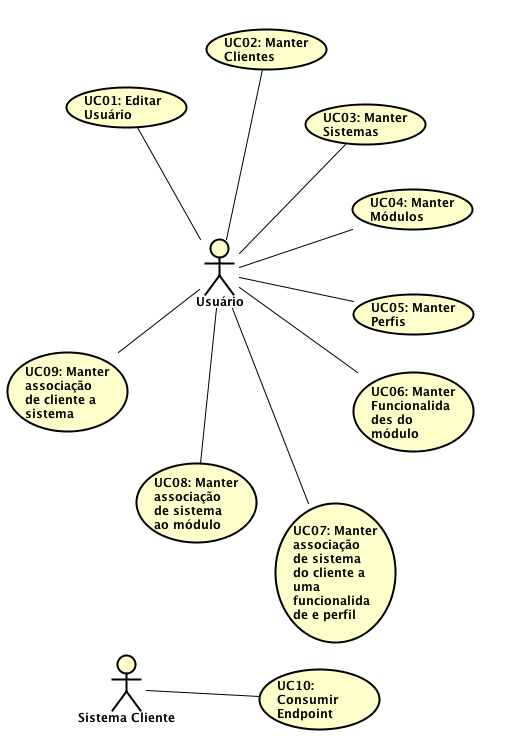
\includegraphics[width=0.8\textwidth]{images/Diagrama_de_caso_de_uso}
	\caption{Diagrama de caso de uso}
    \label{fig:Diagrama de caso de uso}
\end{figure}


Com a figura \ref{fig:Diagrama de classe} é possível compreender com mais clareza o funcionamento do back-end do software, visualizando as classes utilizadas para manipular os dados.

\begin{figure}
	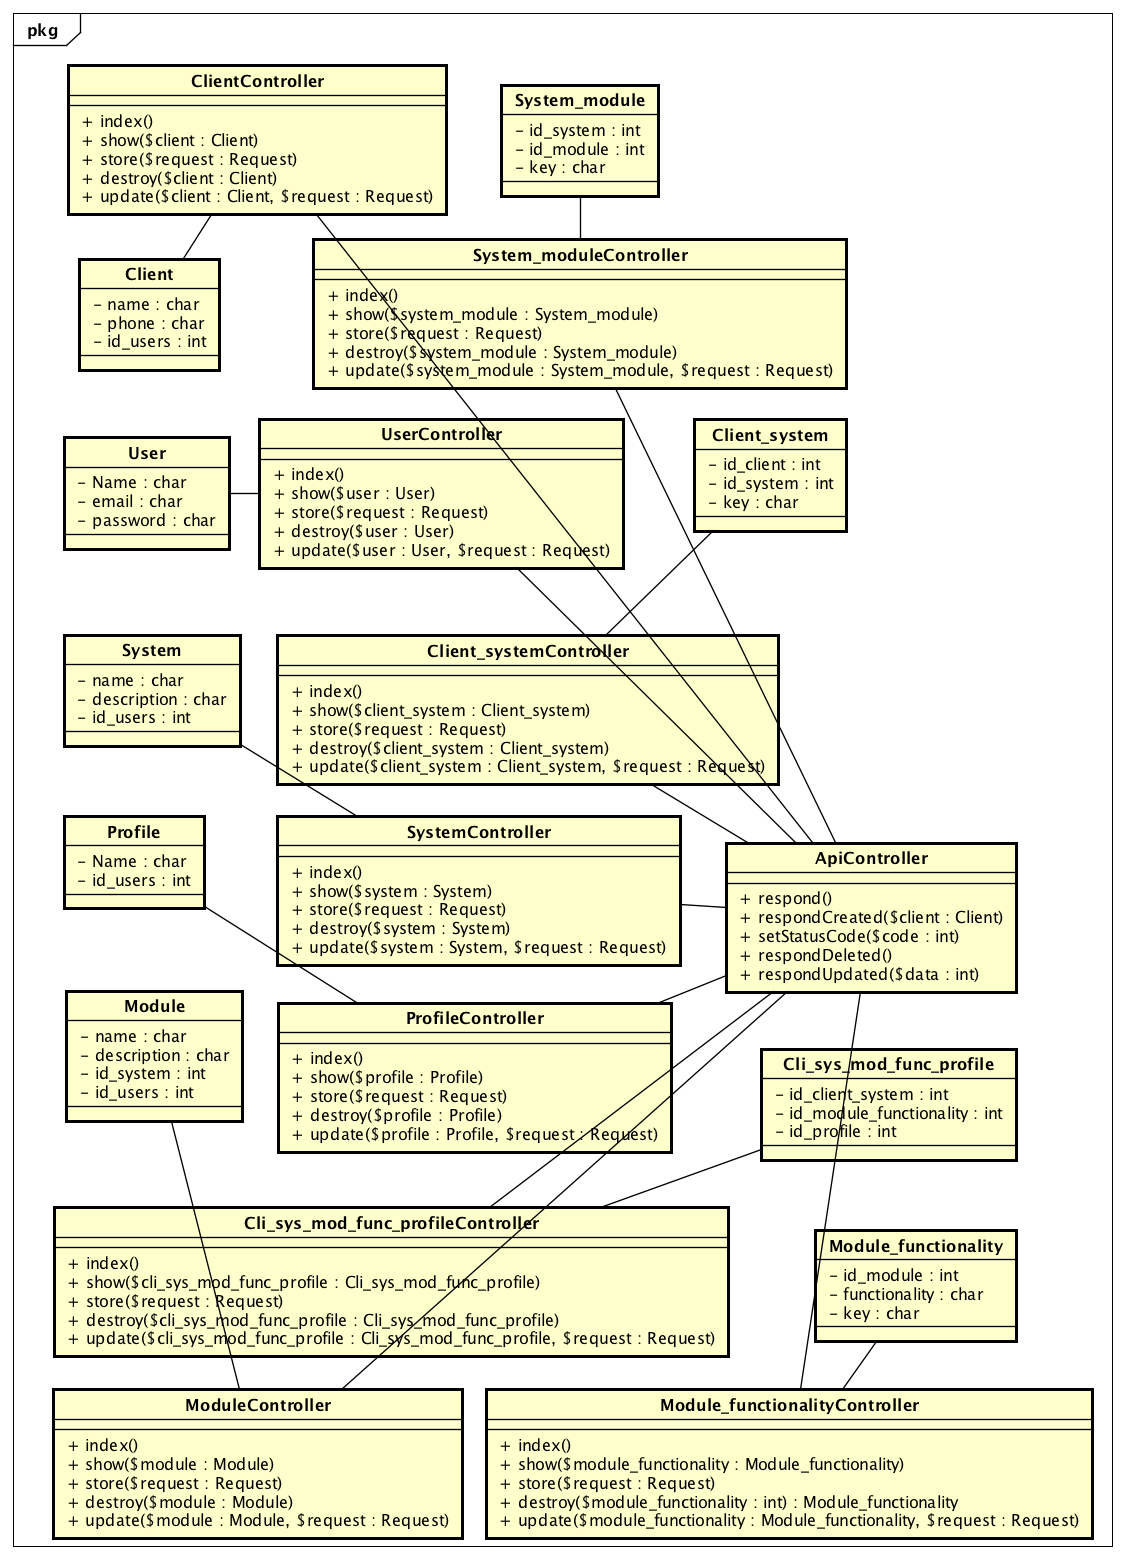
\includegraphics[width=1\textwidth]{images/Diagrama_de_classe}
	\caption{Diagrama de classe}
    \label{fig:Diagrama de classe}
\end{figure}


Por fim, para prover um entendimento de funcionamento interno do software, a figura \ref{fig:DER} traz o diagrama de entidade relacionamento, fornecendo uma ilustração da organização do banco de dados utilizado.


\begin{figure}
	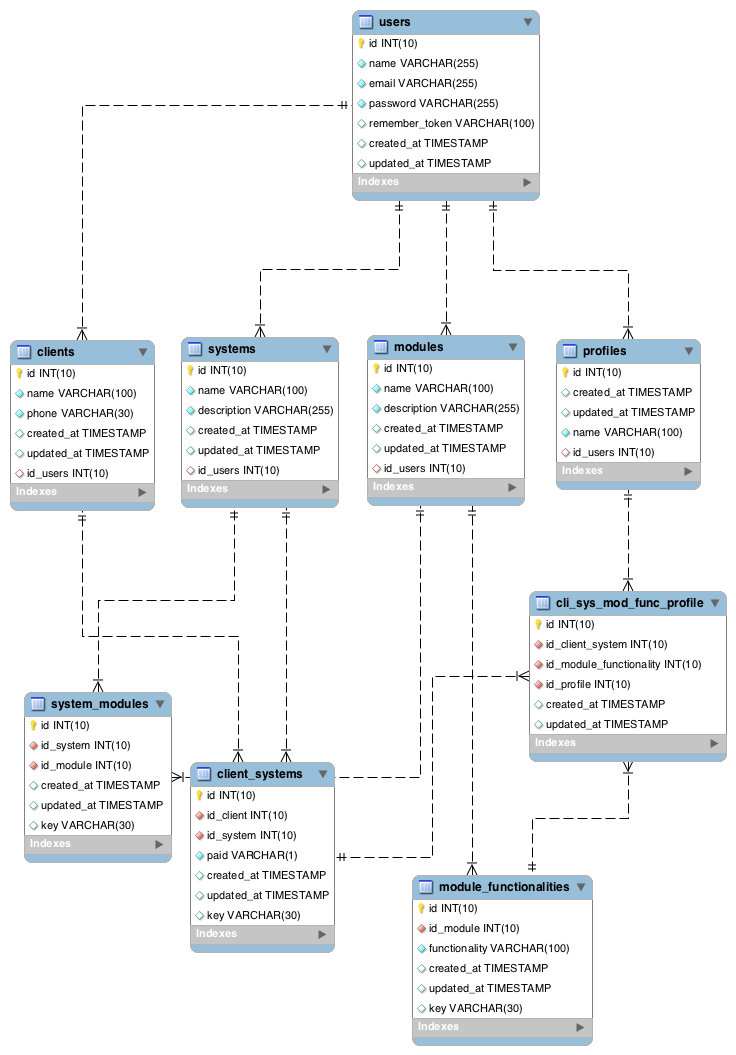
\includegraphics[width=1\textwidth]{images/DER}
	\caption{Diagrama entidade relacionamento}
    \label{fig:DER}
\end{figure}


Relacionando os diagramas apresentados com a Figura \ref{fig:Diagrama da arquitetura}, o diagrama de caso de uso presente na Figura \ref{fig:Diagrama de caso de uso} representa o usuário em ação diante da caixa entitulada "Aplicação Front-end". O diagrama de classes presente na Figura \ref{fig:Diagrama de classe} está relacionado com a caixa entitulada por "Aplicação Back-end(API)" e o DER, representado na Figura \ref{fig:DER}, na caixa "Banco de dados". 
Também, os diagramas UML aqui apresentados estão relacionados entre si. O diagrama de classe está intimamente ligado ao MER, normalmente cada classe está relacionada a uma tabela correspondente no MER. Também, temos que os casos de uso quando codificados, se relacionam com as classes correspondentes do diagrama de classe.


\section{Funcionalidades do ModMan}\label{sec:funcionalidades}


Esta seção apresenta os requisitos funcionais e não-funcionais que foram escritos para o ModMan. Assim, estes requisitos refletem as funcionalidades implementadas.


\subsubsection{Requisitos não funcionais}


\begin{itemize}
	
	
\item RN01: Usuários Simultâneos


Descrição: O sistema deverá suportar processamento multiusuário, ou seja, vários usuários poderão utilizar o sistema simultaneamente. 


\item RN02: Segurança 


Descrição: O sistema só permitirá acesso aos dados com autorização. Os usuários deverão se identificar usando um login e uma senha, e a referida senha será criptografada com a metodologia Bcrypt no banco de dados.


\end{itemize}
	

\subsubsection{Requisitos funcionais}


\begin{itemize}
	
	
\item RF 01: Login


Descrição: O sistema deve conter tela de login com os campos email e senha. Após inserção dos dados, o sistema deve validar os dados e caso positivo, encaminhar o usuário ao sistema. Caso os dados sejam inválidos, exibir mensagem de erro para o usuário.


\item RF 02: Edição de usuário


Descrição: O sistema deve conter um formulário que seja carregado com os dados do usuário da sessão e permitir a atualização dos dados. Este requisito está relacionado ao UC01 da figura \ref{fig:Diagrama de caso de uso}.


\item RF 03: Cadastro de cliente


Descrição: O sistema deve conter um formulário para cadastro de clientes. Após a inserção de um registro, o sistema deve automaticamente exibir o registro em formato de edição e conter botão para ir a uma consulta que liste os clientes cadastrados para o usuário da sessão. Este requisito está relacionado ao UC02 da figura \ref{fig:Diagrama de caso de uso}.


\item RF 04: Cadastro de sistema


Descrição: O sistema deve conter um formulário para cadastro de sistemas. Após a inserção de um registro, o sistema deve automaticamente exibir o registro em formato de edição e conter botão para ir a uma consulta que liste os sistemas cadastrados para o usuário da sessão. Este requisito está relacionado ao UC03 da figura \ref{fig:Diagrama de caso de uso}.


\item RF 05: Cadastro de módulo


Descrição: O sistema deve conter um formulário para cadastro de módulos. Após a inserção de um registro, o sistema deve automaticamente exibir o registro em formato de edição e conter botão para ir a uma consulta que liste os módulos cadastrados para o usuário da sessão. Este requisito está relacionado ao UC04 da figura \ref{fig:Diagrama de caso de uso}.


\item RF 06: Cadastro de perfil


Descrição: O sistema deve conter um formulário para cadastro de perfil. Após a inserção de um registro, o sistema deve automaticamente exibir o registro em formato de edição e conter botão para ir a uma consulta que liste os perfils cadastrados para o usuário da sessão. Este requisito está relacionado ao UC05 da figura \ref{fig:Diagrama de caso de uso}.\linebreak


\item RF 07: Cadastro associativo de cliente aos sistemas


Descrição: O sistema deve conter um formulário para cadastro associativo de clientes a sistemas. Após a inserção de um registro, o sistema deve automaticamente gerar uma chave de acesso do dado registro para o usuário consultar permissões e exibir o registro em formato de edição e conter botão para ir a uma consulta que liste os registros associativos de clientes aos sistemas cadastrados para o usuário da sessão. Este requisito está relacionado ao UC09 da figura \ref{fig:Diagrama de caso de uso}.


\item RF 08: Cadastro associativo de  sistemas aos módulos


Descrição: O sistema deve conter um formulário para cadastro associativo de sistemas a módulos. Após a inserção de um registro, o sistema deve automaticamente gerar uma chave de acesso do dado registro para o usuário consultar permissões e exibir o registro em formato de edição e conter botão para ir a uma consulta que liste os registros associativos de  sistemas aos módulos cadastrados para o usuário da sessão. Este requisito está relacionado ao UC08 da figura \ref{fig:Diagrama de caso de uso}.


\item RF 09: Cadastro de funcionalidade dos módulos


Descrição: O sistema deve conter um formulário para cadastro de funcionalidade dos módulos já cadastrados. Após a inserção de um registro, o sistema deve automaticamente gerar uma chave de acesso do dado registro para o usuário consultar permissões e exibir o registro em formato de edição e conter botão para ir a uma consulta que liste os registros de funcionalidades cadastradas para o usuário da sessão. Este requisito está relacionado ao UC06 da figura \ref{fig:Diagrama de caso de uso}.


\item RF 10: Composição de permissão para os módulos dos clientes


Descrição: O sistema deve conter um formulário para cadastro associativo de permissão para os módulos dos clientes. Após a inserção de um registro, o sistema deve automaticamente exibir o registro em formato de edição e conter botão para ir a uma consulta que liste os registros associativos de permissão cadastrados para o usuário da sessão. Este requisito está relacionado ao UC07 da figura \ref{fig:Diagrama de caso de uso}.


\item RF 11: Endpoint


Descrição: O sistema deve disponibilizar a URL http://api.modman.ga/api/endpoint para receber uma requisição via post, que deve receber um parâmetro "key" contendo a chave de acesso desejada para consultar as permissões cadastradas. Ao realizar a requisiçao enviando a "key", o sistema deve retornar um texto no formato Json, contendo os dados das permissões que foram compostas no sistema pelo usuário. A chave enviada pelo usuário pode ser de qualquer um dos níveis de configuração realizado no sistema e o o endpoint deve retornar a resposta sempre num mesmo formato, viabilizando um tratamento único da resposta pelo cliente. Este requisito está relacionado ao UC10 da figura \ref{fig:Diagrama de caso de uso}.


\end{itemize}


Para melhor compreensão do sistema proposto, a Figura \ref{fig:diagramaBpmn} apresenta uma visão geral do processo implementado na ferramenta, utilizando, para tal, a notação BPMN (Business Process Model and Notation).


\begin{figure} %\landscape 
	%\vspace*{-2cm}
	\makebox[\linewidth]{
		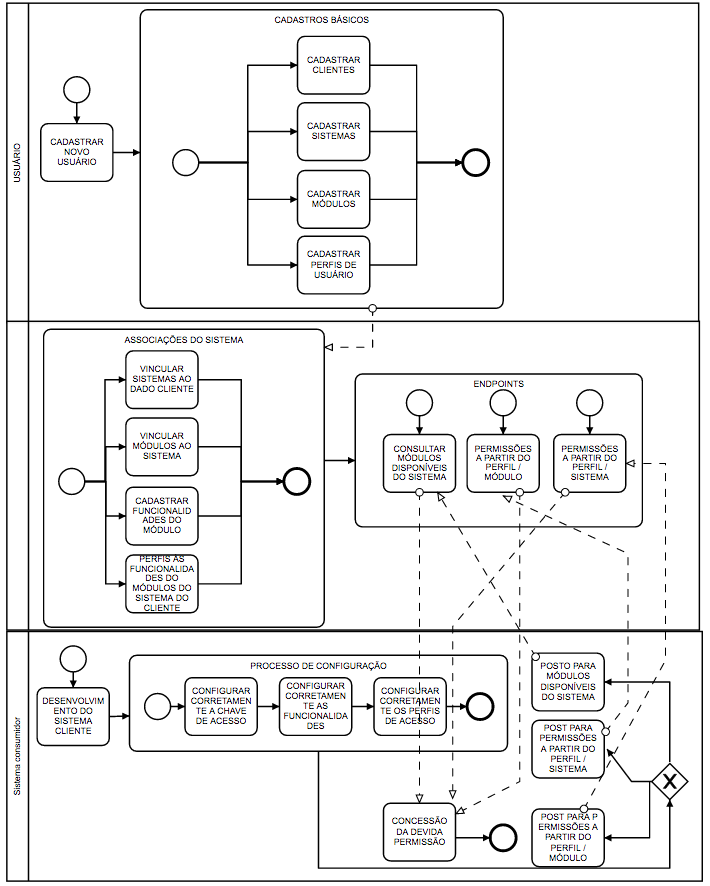
\includegraphics[width=1.2\linewidth]{images/diagrama_bpmn}
	}
	\caption{Diagrama do processo do ModMan}
    \label{fig:diagramaBpmn}
\end{figure}


\section{Resumo do capítulo}\label{sec:resumo} %Sob o ponto de vista tecnológico


Seguindo a norma de padronização de código, com o ModMan é possível unificar o módulo de permissões de acesso e tratá-lo como um serviço, tornando possível eliminá-lo de qualquer software que faça uso do mesmo. A proposta trata de uma aplicabilidade diferente do controle de permissão dos perfis, que não foi detectada em sistemas disponíveis no estado da prática.

Os artefatos de software aqui apresentados servem para embasar qualquer usuário do ModMan, pois será possível tomar conhecimento sobre a razão da escolha das tecnologias utilizadas, da arquitetura, mapeando vantagens e desvantagens e também tomar conhecimento da proposta de cada funcionalidade do sistema através dos requisitos funcionais. Complementando o entendimento, os diagramas UML fornecem melhor visão de determinados aspectos, a exemplo do diagrama de classe que exibe a organização interna das classes do back-end do software.